\documentclass[12pt]{article}

\usepackage[utf8]{inputenc}
\usepackage{amsmath}
\usepackage{graphicx}
\usepackage{titlesec}
\usepackage{tcolorbox}
\usepackage{amssymb}
\usepackage{wrapfig}

\title{\bfseries Laborator Electricitate 2}
\author{Sîrghe Matei}
\date{\today}

\titleformat{\section}
  {\normalfont\Large\bfseries}{\thesection}{1em}{}

\begin{document}

\maketitle

\section{Teoria Lucrării}
Putem depista experimental dacă un obiect este electrizat cu ajutorul electroscopului. Dacă electroscopul se descarcă, atunci obiectul este electrizat.

\section{Electroscopul}

\begin{wrapfigure}{r}{0.5\textwidth} % 'r' for right, '0.4\textwidth' for 40% of the text width
    \centering
    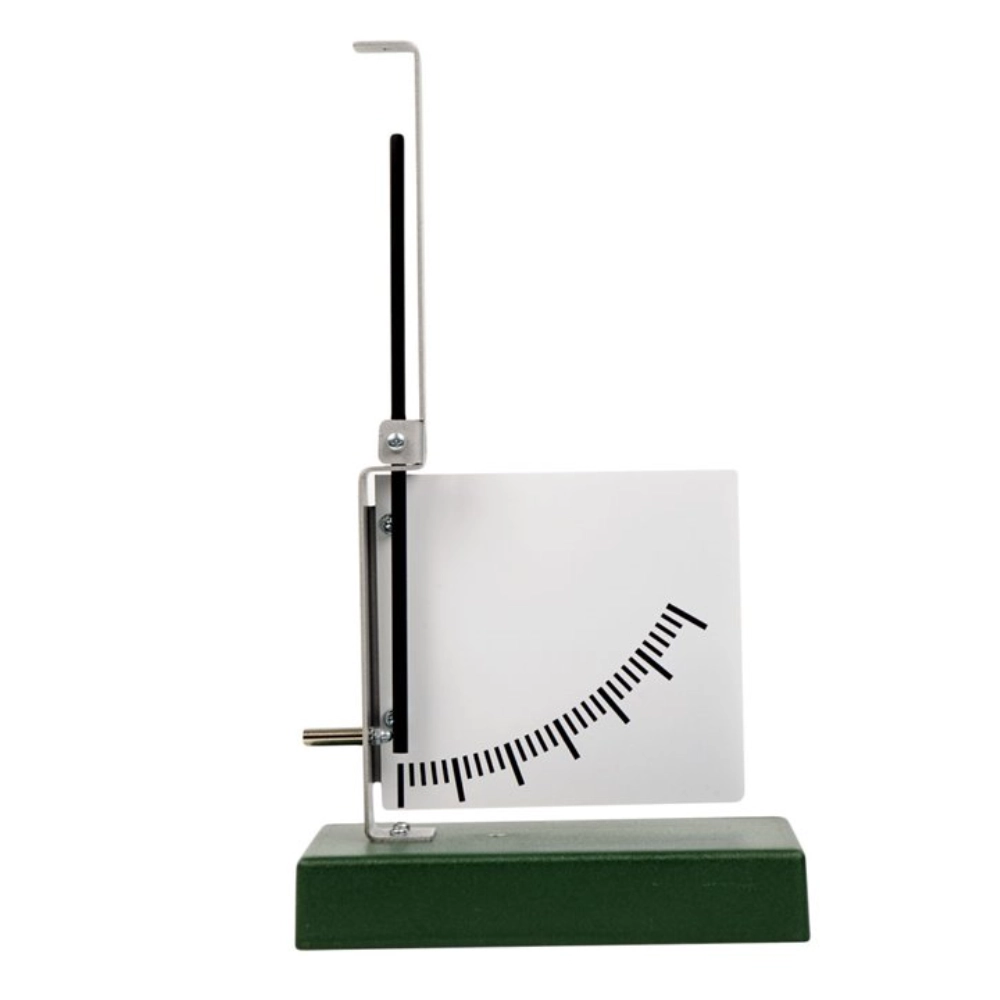
\includegraphics[width=0.38\textwidth]{electroscop.png} % Adjust the width as needed
    \caption{Imaginea unui electroscop}
    \label{fig:electroscop}
\end{wrapfigure}

Dacă frecăm cu cârpa un material izolator și apropiem materialul de electroscop, constatăm că acul electroscopului deviază. Există doua feluri
de sarcină electrică numite pozitivă și negativă care interacționează astfel.

\[
\oplus \rightarrow \leftarrow \ominus \quad 
\quad \oplus \leftarrow \rightarrow \oplus \quad 
\quad \ominus \leftarrow \rightarrow \ominus
\]


Plus cu plus se resping.

Minus cu minus se resping.

Plus cu minus se atrag.
\section{Electrizarea}
Izolatoarele nu sunt toate la fel de bune. De exemplu, aerul este un izolator mai bun decât hartia. Metalele se comportă diferit față de Izolatoarele
deoarece au înăuntru lor electroni liberi când izolatoarele au foarte puțini electroni liberi.
Cu ajutorul fizicii moderne, putem explica foarte ușor de ce deviază acul electroscopului. Să presupunem că apropiem un corp electrizat pozitiv
de electroscop. 

Electronii liberi din bila eletroscopului, din tija metalică groasă și din acul subțire metalic sunt atrași de către corpul pozitiv
înspre partea superioară a electroscopului. În timpul mișcării, locul de unde pleacă acești electroni rămâne încărcat pozitiv , inclusiv capătul
de jos al tijei și capătul de jos al acului metalic. În consecință , + cu  + se va respinge și acul deviază. Nu putem afla semnul sarcinii doar
cu electroscopul. El ne indică doar dacă un obiect este electrizat sau nu.

\end{document}